\documentclass[]{article}
\usepackage{lmodern}
\usepackage{amssymb,amsmath}
\usepackage{ifxetex,ifluatex}
\usepackage{fixltx2e} % provides \textsubscript
\ifnum 0\ifxetex 1\fi\ifluatex 1\fi=0 % if pdftex
  \usepackage[T1]{fontenc}
  \usepackage[utf8]{inputenc}
\else % if luatex or xelatex
  \ifxetex
    \usepackage{mathspec}
  \else
    \usepackage{fontspec}
  \fi
  \defaultfontfeatures{Ligatures=TeX,Scale=MatchLowercase}
\fi
% use upquote if available, for straight quotes in verbatim environments
\IfFileExists{upquote.sty}{\usepackage{upquote}}{}
% use microtype if available
\IfFileExists{microtype.sty}{%
\usepackage{microtype}
\UseMicrotypeSet[protrusion]{basicmath} % disable protrusion for tt fonts
}{}
\usepackage[margin=1in]{geometry}
\usepackage{hyperref}
\hypersetup{unicode=true,
            pdftitle={Coupled predator-prey models and its application in investing in stock market},
            pdfauthor={Aurél György Prósz, XGRP0J},
            pdfborder={0 0 0},
            breaklinks=true}
\urlstyle{same}  % don't use monospace font for urls
\usepackage{graphicx,grffile}
\makeatletter
\def\maxwidth{\ifdim\Gin@nat@width>\linewidth\linewidth\else\Gin@nat@width\fi}
\def\maxheight{\ifdim\Gin@nat@height>\textheight\textheight\else\Gin@nat@height\fi}
\makeatother
% Scale images if necessary, so that they will not overflow the page
% margins by default, and it is still possible to overwrite the defaults
% using explicit options in \includegraphics[width, height, ...]{}
\setkeys{Gin}{width=\maxwidth,height=\maxheight,keepaspectratio}
\IfFileExists{parskip.sty}{%
\usepackage{parskip}
}{% else
\setlength{\parindent}{0pt}
\setlength{\parskip}{6pt plus 2pt minus 1pt}
}
\setlength{\emergencystretch}{3em}  % prevent overfull lines
\providecommand{\tightlist}{%
  \setlength{\itemsep}{0pt}\setlength{\parskip}{0pt}}
\setcounter{secnumdepth}{0}
% Redefines (sub)paragraphs to behave more like sections
\ifx\paragraph\undefined\else
\let\oldparagraph\paragraph
\renewcommand{\paragraph}[1]{\oldparagraph{#1}\mbox{}}
\fi
\ifx\subparagraph\undefined\else
\let\oldsubparagraph\subparagraph
\renewcommand{\subparagraph}[1]{\oldsubparagraph{#1}\mbox{}}
\fi

%%% Use protect on footnotes to avoid problems with footnotes in titles
\let\rmarkdownfootnote\footnote%
\def\footnote{\protect\rmarkdownfootnote}

%%% Change title format to be more compact
\usepackage{titling}

% Create subtitle command for use in maketitle
\newcommand{\subtitle}[1]{
  \posttitle{
    \begin{center}\large#1\end{center}
    }
}

\setlength{\droptitle}{-2em}

  \title{Coupled predator-prey models and its application in investing in stock
market}
    \pretitle{\vspace{\droptitle}\centering\huge}
  \posttitle{\par}
    \author{Aurél György Prósz, XGRP0J}
    \preauthor{\centering\large\emph}
  \postauthor{\par}
      \predate{\centering\large\emph}
  \postdate{\par}
    \date{2018 október 9}


\begin{document}
\maketitle

{
\setcounter{tocdepth}{2}
\tableofcontents
}
\section{Introduction}\label{introduction}

Predator-prey models are important topics not only in biology, but in
other fields like plasma
physics{[}\url{http://iopscience.iop.org/article/10.1088/0741-3335/56/1/015002}{]},
economics{[}\url{https://www.sciencedirect.com/science/article/pii/0895717794900124}{]},
or even in criminology
{[}\url{https://www.ncbi.nlm.nih.gov/pmc/articles/PMC5043299/}{]}.\\
The first, simplest model originated from the study of fish populations
of the Mediterranean after the first world war, by Lotka and Volterra.
In their model there are two types of species: the prey, and the
predator. They form a simple food-chain where the predator species hunts
the prey species, while the prey grazes vegetation. Their behavior and
the time evolution of the number of species are characterized by a
simple system of two, nonlinear first order differential equations. By
solving these equations we can have insights on how the number of
predators and preys evolve in time.\\
In this document I present the classical Lotka-Volterra (LV) equations
and its modified versions. I also reproduce a financial model described
in {[}\url{https://ijpam.eu/contents/2016-107-2/17/17.pdf}{]}, which can
be used by a stock market trader to eliminate some of its risks
involving the trading of specific stocks by buying the shares of so
called prey companies, and sell them to a predator company.

\section{Project goals}\label{project-goals}

Implement and interpret the:

\begin{itemize}
\tightlist
\item
  Classical LV model
\item
  Classical LV model at equilibrium
\item
  LV model with prey hill function and LV model with predator efficiency
\item
  LV model with one predator - two preys without interaction between the
  preys
\item
  LV model used in stock market
\end{itemize}

\subsection{My own contribution to the
topic}\label{my-own-contribution-to-the-topic}

The first three models are discussed in the {[}willeybook{]} already,
but was implemented in Python. My own contribution to these tasks is to
recreate them using R and its DeSolve library and to validate my further
results.\\
The one predator - two preys model was discussed in {[}{]} and {[}{]},
but with an interaction term included between the preys, so I found it
interesting if I can analyze the results without the interactions.

\section{Materials and methods}\label{materials-and-methods}

\subsection{R programming language}\label{r-programming-language}

R is a language and environment for statistical computing and graphics.
It is a GNU project which is similar to the S language and environment
which was developed at Bell Laboratories (formerly AT\&T, now Lucent
Technologies) by John Chambers and colleagues. R provides a wide variety
of statistical (linear and nonlinear modelling, classical statistical
tests, time-series analysis, classification, clustering, \ldots{}) and
graphical techniques, and is highly extensible.

\subsection{DeSolve library}\label{desolve-library}

R package deSolve is the successor of R package odesolve, which is a
package to solve initial value problems (IVP) of ordinary differential
equations (ODE), differential algebraic equations (DAE), partial
differential equations (PDE), and delay differential equations (DeDE). I
used this package to solve the systems of nonlinear differential
equations present in predator-prey models.\\
The particular function I used for the solutions is the \emph{lsoda}
function {[}{]}.

\subsection{Possible source of errors}\label{possible-source-of-errors}

\section{Classical LV model}\label{classical-lv-model}

This model describes the interaction of a predatory and a prey species.
The predators try to catch the preys, thus increasing their population,
and decreasing the prey's. In this model the prey species has unlimited
resources to feed, and in this way the population of the prey species
grows exponentially if no predatory species are present. We can
summarize the whole model in a system of nonlinear differential
equations: \[
\frac{dX}{dt}= aX-bXY
\] \[
\frac{dY}{dt}= bkXY-lY
\] where \emph{x} and \emph{y} are the prey and predator density,
respectively, \emph{a} and \emph{l} determines how fast the preys
reproduce and the predators die of hunger. \emph{b} and \emph{k}
describes the interaction part of the equation, where \emph{b} governs
the interaction rate between the two species, and \emph{k} is set the
efficiency of which the predators converts prey to food.

\includegraphics{project_markdown_files/figure-latex/unnamed-chunk-1-1.pdf}

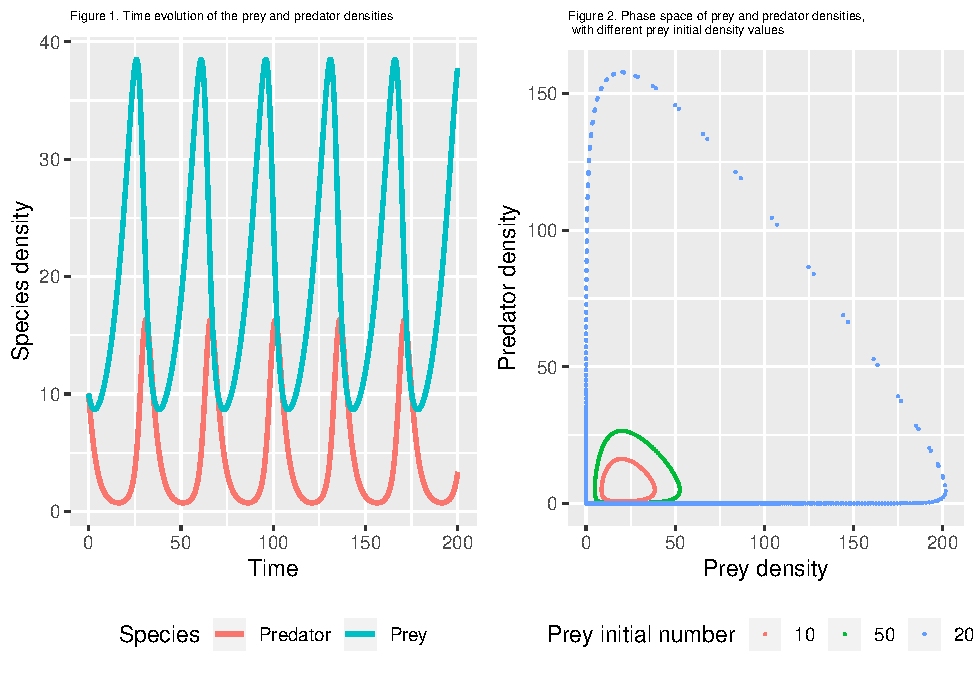
\includegraphics{project_markdown_files/figure-latex/unnamed-chunk-2-1.pdf}

\subsection{Discussion}\label{discussion}

On plot1 one can see that the solution of this model is an oscillatory
behavior, where the prey and predator density rise and fall out of phase
respect to each other.Plotting the x,y phase space on plot2 shows closed
orbits, called limit cycles. However, the orbits are not perfectly
closed due to the errors in the numerical integration of the equations.

\section{LV model with prey limit and predator
efficiency}\label{lv-model-with-prey-limit-and-predator-efficiency}

This model extends the classical LV model in such a way, that it
includes a so called K carrying capacity for the prey population, and a
functional response palpha, as the probability a predator finds one
prey. These two parameters makes the model more realistic, as in reality
the resources available for the preys are not unlimited, and the hunt by
the predators are not always successful, and takes time. \[
\frac{dX}{dt} = Xa(1-\frac{X}{K}) - \frac{bYX}{1+bX\tau}
\] \[
\frac{dY}{dt}= bkXY-lY
\]

\includegraphics{project_markdown_files/figure-latex/unnamed-chunk-3-1.pdf}
\includegraphics{project_markdown_files/figure-latex/unnamed-chunk-3-2.pdf}

Equation Source of errors Pictures

\section{Two preys, one predator LV
model}\label{two-preys-one-predator-lv-model}

This modification of the original LV model includes the extensions
mentioned above, and also includes one more prey species. In reality
there can be preys which can be hunted down more easily by the predator,
and could have different carrying capacity. These biological information
are included in the parameters of this model.

\$\$ \frac{dX_{1}}{dt} = Xa\_\{1\}(1-\frac{X_{1}}{K_{1}}) -
\frac{b_{1}YX_{1}}{1+b_{1}X_{1}\tau_{1}}

\[
\] \frac{dX_{2}}{dt} = Xa\_\{2\}(1-\frac{X_{2}}{K_{2}}) -
\frac{b_{2}YX_{2}}{1+b_{2}X_{2}\tau_{2}} \$\$

\[
\frac{dY}{dt}= \delta X_{1}Y + \delta X_{2}Y-lY
\]

\includegraphics{project_markdown_files/figure-latex/unnamed-chunk-4-1.pdf}

\section{Stock market application}\label{stock-market-application}

Within recent times, application of models which originate from biology
have become used in finance to describe the complex behavior of the
stock market. There are multiple approaches {[}{]} which tries to apply
the slightly modified version of the predator-prey models to analyze how
venture capital investments exhaust the available stock of
opportunities. A trader would be likely to make a more informed choice
between competing stocks or shares based on comparisons among prices per
share.\\
In the model described in this chapter the financially powerful trading
company who wants to acquire smaller, financially weak companies, is the
predator, while the smaller companies represent the prey. The predator
makes a monetary offer for the prey shares. Once purchased, these shares
are held until they are converted to predator shares.\\
The main objective is to simulate the system described above, and to
make profit from the price changes.\\
In order for this to be profitable financially, the predator needs to
have an estimate of the risk involved in this trade and this is based on
changes in his predatory share prices.\\
Analyzing the simulation results can allow the trader to find the
specific parameters which makes the system stable, and this would allow
determine if the acquistion of prey company shares is profitable, or
not.\\
\[
\frac{X_{1}}{dt} = \alpha_{1}X_{1}\left ( 1-\frac{X_{1}}{K_{1}} \right )-m_{12}X_{1}X_{2} - \beta X_{1}Yr_{1}
\]

\[
\frac{X_{2}}{dt} = \alpha_{2}X_{2}\left ( 1-\frac{X_{2}}{K_{2}} \right )-m_{21}X_{1}X_{2} - \beta X_{2}Yr_{2}
\]

\[
\frac{dY}{dt} = -\mu Y + c_{1}\beta_{1}X_{1}Yr_{1} + c_{2}\beta_{2}X_{2}Yr_{2}
\]

\[
r1 = \frac{1}{1+\left ( \frac{a_{2}X_{2}+b_{2}Y}{X_{1}} \right )^{n}}
\]

\[
r2 = \frac{1}{1+\left ( \frac{a_{1}X_{1}+b_{1}Y}{X_{2}} \right )^{n}}
\]

\emph{X1} and \emph{X2} are relative share prices of competing prey
companies, \emph{Y} is the relative price per share of the predator
company. The parameters used in the model are all non-negative.\\
\emph{alpha1} and \emph{alpha2}: Intrinsic growth rate of prey share
price,\\
\emph{K1} and \emph{K2}: Carrying capacity of prey shares,\\
\emph{m12} and \emph{m21}: Inter-specific competition between prey
market shares,\\
\emph{beta1} and \emph{beta2}: Predatory capture rate is the probability
predator Y invests in prey X1 or X2,\\
\emph{a1} and \emph{a2}: Harvesting rate of prey shares,\\
\emph{b1} and \emph{b2}: Anti-predator behavior of prey shares,\\
\emph{c1} and \emph{c2}: Rate of conversion of prey shares to predator
shares,\\
\emph{mu}: Rate of decline of predator share price,\\
\emph{n} : Multiplicative effect due to the predatory functional
response.

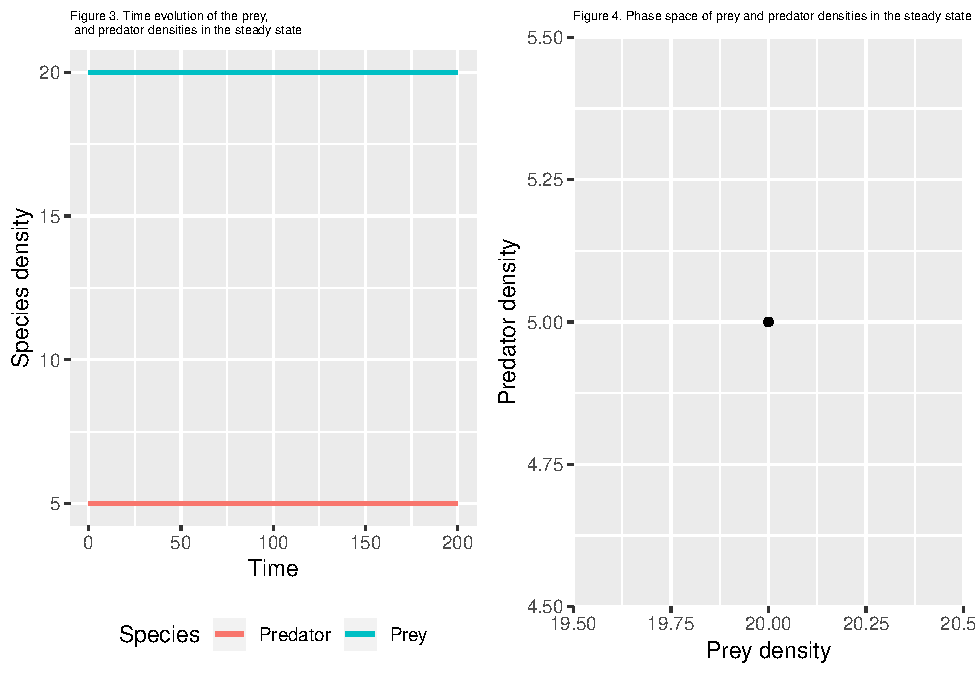
\includegraphics{project_markdown_files/figure-latex/unnamed-chunk-5-1.pdf}


\end{document}
